\chapter{Errata list}\label{errata}

\begin{itemize}
    \item p.101. eq (2.150) $\rho = \sum_m p(m) \rho_m$ should be $\rho \textcolor{red}{'} = \sum_m p(m) \rho_m$.
%
  \item p.103. Exercise 2.26. Show that the circuit:
\begin{center}
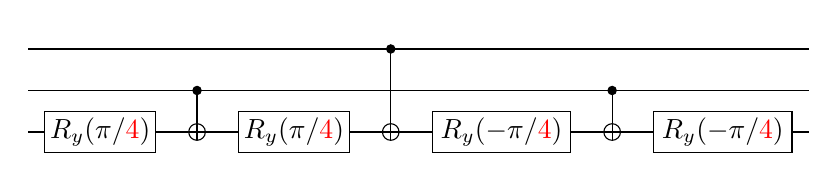
\begin{tikzpicture}[scale=1.000000,x=1pt,y=1pt]
\filldraw[color=white] (0.000000, -7.500000) rectangle (282.000000, 37.500000);
% Drawing wires
% Line 1: a3 W
\draw[color=black] (0.000000,30.000000) -- (282.000000,30.000000);
% Line 2: a2 W
\draw[color=black] (0.000000,15.000000) -- (282.000000,15.000000);
% Line 3: a1 W
\draw[color=black] (0.000000,0.000000) -- (282.000000,0.000000);
% Done with wires; drawing gates
% Line 4: a1 G $R_y(\pi/\textcolor{red}{4})$ width=40 height=15
\begin{scope}
\draw[fill=white] (26.000000, -0.000000) +(-45.000000:28.284271pt and 10.606602pt) -- +(45.000000:28.284271pt and 10.606602pt) -- +(135.000000:28.284271pt and 10.606602pt) -- +(225.000000:28.284271pt and 10.606602pt) -- cycle;
\clip (26.000000, -0.000000) +(-45.000000:28.284271pt and 10.606602pt) -- +(45.000000:28.284271pt and 10.606602pt) -- +(135.000000:28.284271pt and 10.606602pt) -- +(225.000000:28.284271pt and 10.606602pt) -- cycle;
\draw (26.000000, -0.000000) node {$R_y(\pi/\textcolor{red}{4})$};
\end{scope}
% Line 5: +a1 a2
\draw (61.000000,15.000000) -- (61.000000,0.000000);
\begin{scope}
\draw[fill=white] (61.000000, 0.000000) circle(3.000000pt);
\clip (61.000000, 0.000000) circle(3.000000pt);
\draw (58.000000, 0.000000) -- (64.000000, 0.000000);
\draw (61.000000, -3.000000) -- (61.000000, 3.000000);
\end{scope}
\filldraw (61.000000, 15.000000) circle(1.500000pt);
% Line 6: a1 G $R_y(\pi/\textcolor{red}{4})$ width=40 height=15
\begin{scope}
\draw[fill=white] (96.000000, -0.000000) +(-45.000000:28.284271pt and 10.606602pt) -- +(45.000000:28.284271pt and 10.606602pt) -- +(135.000000:28.284271pt and 10.606602pt) -- +(225.000000:28.284271pt and 10.606602pt) -- cycle;
\clip (96.000000, -0.000000) +(-45.000000:28.284271pt and 10.606602pt) -- +(45.000000:28.284271pt and 10.606602pt) -- +(135.000000:28.284271pt and 10.606602pt) -- +(225.000000:28.284271pt and 10.606602pt) -- cycle;
\draw (96.000000, -0.000000) node {$R_y(\pi/\textcolor{red}{4})$};
\end{scope}
% Line 7: +a1 a3
\draw (131.000000,30.000000) -- (131.000000,0.000000);
\begin{scope}
\draw[fill=white] (131.000000, 0.000000) circle(3.000000pt);
\clip (131.000000, 0.000000) circle(3.000000pt);
\draw (128.000000, 0.000000) -- (134.000000, 0.000000);
\draw (131.000000, -3.000000) -- (131.000000, 3.000000);
\end{scope}
\filldraw (131.000000, 30.000000) circle(1.500000pt);
% Line 8: a1 G $R_y(-\pi/\textcolor{red}{4})$ width=50 height=15
\begin{scope}
\draw[fill=white] (171.000000, -0.000000) +(-45.000000:35.355339pt and 10.606602pt) -- +(45.000000:35.355339pt and 10.606602pt) -- +(135.000000:35.355339pt and 10.606602pt) -- +(225.000000:35.355339pt and 10.606602pt) -- cycle;
\clip (171.000000, -0.000000) +(-45.000000:35.355339pt and 10.606602pt) -- +(45.000000:35.355339pt and 10.606602pt) -- +(135.000000:35.355339pt and 10.606602pt) -- +(225.000000:35.355339pt and 10.606602pt) -- cycle;
\draw (171.000000, -0.000000) node {$R_y(-\pi/\textcolor{red}{4})$};
\end{scope}
% Line 9: +a1 a2
\draw (211.000000,15.000000) -- (211.000000,0.000000);
\begin{scope}
\draw[fill=white] (211.000000, 0.000000) circle(3.000000pt);
\clip (211.000000, 0.000000) circle(3.000000pt);
\draw (208.000000, 0.000000) -- (214.000000, 0.000000);
\draw (211.000000, -3.000000) -- (211.000000, 3.000000);
\end{scope}
\filldraw (211.000000, 15.000000) circle(1.500000pt);
% Line 10: a1 G $R_y(-\pi/\textcolor{red}{4})$ width=50 height=15
\begin{scope}
\draw[fill=white] (251.000000, -0.000000) +(-45.000000:35.355339pt and 10.606602pt) -- +(45.000000:35.355339pt and 10.606602pt) -- +(135.000000:35.355339pt and 10.606602pt) -- +(225.000000:35.355339pt and 10.606602pt) -- cycle;
\clip (251.000000, -0.000000) +(-45.000000:35.355339pt and 10.606602pt) -- +(45.000000:35.355339pt and 10.606602pt) -- +(135.000000:35.355339pt and 10.606602pt) -- +(225.000000:35.355339pt and 10.606602pt) -- cycle;
\draw (251.000000, -0.000000) node {$R_y(-\pi/\textcolor{red}{4})$};
\end{scope}
% Done with gates; drawing ending labels
% Done with ending labels; drawing cut lines and comments
% Done with comments
\end{tikzpicture}
\end{center}
\vspace{-5pt}
differs from a Toffoli gate only by relative phases.

    \item p.408. eq (9.49) $\sum_i p_i D(\rho_i, \sigma_i) + D(p_i, q_i)$ should be $\sum_i p_i D(\rho_i, \sigma_i) + \textcolor[rgb]{1,0,0}{2}D(p_i, q_i)$.

    \begin{align*}
    \text{eqn } (9.48) 
        &= \sum_i p_i \Tr (P(\rho_i - \sigma_i)) + \sum_i (p_i - q_i) \Tr (P \sigma_i)\\
        &\leq \sum_i p_i \Tr (P(\rho_i - \sigma_i)) + \sum_i |p_i - q_i| \Tr (P \sigma_i)~~~(\because p_i - q_i \leq |p_i - q_i|)\\
        &\leq \sum_i p_i \Tr (P(\rho_i - \sigma_i)) + \sum_i |p_i - q_i|~~~(\because \Tr (P \sigma_i) \leq 1)\\
        &= \sum_i p_i \Tr (P(\rho_i - \sigma_i)) + 2 \frac{\sum_i |p_i - q_i|}{2}\\
        &= \sum_i p_i \Tr (P(\rho_i - \sigma_i)) + 2D(p_i, q_i)
    \end{align*}
%
    \item p.409. Exercise 9.12. If $\rho = \sigma$, then $D(\rho, \sigma) = 0$. Furthermore trace distance is non-negative. Therefore $0 \leq D(\mathcal{E}(\rho), \mathcal{E}(\sigma)) \leq 0 \Rightarrow D(\mathcal{E}(\rho), \mathcal{E}(\sigma))  = 0$. So I think the map $\mathcal{E}$ is not strictly contractive. If $p \neq 1$ and $\rho \neq \sigma$, then $D(\mathcal{E}(\rho), \mathcal{E}(\sigma)) < D(\rho, \sigma)$ is satisfied.
%
    \item p.411. Exercise 9.16. eqn(9.73) $\Tr (A^\dagger B) = \braket{m | A \otimes B | m}$ should be $\Tr (A^{\textcolor{red}{T}} B) = \braket{m | A \otimes B | m}$.

    Simple counter example is the case that
    $A = \begin{bmatrix}
        i & 0\\
        0 & 0
    \end{bmatrix}$.
    $B = \begin{bmatrix}
        1 & 0\\
        0 & 0
    \end{bmatrix}$,
    In this case,
    \begin{align*}
        A^\dagger B &=
        \begin{bmatrix}
            -i & 0\\
            0 & 0
        \end{bmatrix}
        \begin{bmatrix}
            1 & 0\\
            0 & 0
        \end{bmatrix}
        = \begin{bmatrix}
            -i & 0\\
            0 & 0
        \end{bmatrix},\\
%
        \Tr (A^\dagger B)& = -i,\\
%
        A \otimes B &= \begin{bmatrix}
            i & 0 & 0 & 0\\
            0 & 0 & 0 & 0\\
            0 & 0 & 0 & 0\\
            0 & 0 & 0 & 0
        \end{bmatrix}\\
        \braket{m | A \otimes B | m} &= (\bra{00} + \braket{11}) (A \otimes B) (\ket{00} + \ket{11}) = i.
    \end{align*}
    Thus $\Tr(A^\dagger B) \neq \braket{m | A \otimes B | m}$.

    By using following relation, we can prove.
    \begin{align*}
        (I \otimes A) \ket{m} = (A^T \otimes I) \ket{m}\\
        \Tr (A) = \braket{m | I \otimes A | m}
    \end{align*}
%
    \begin{align*}
        \Tr (A^T B) = \Tr(BA^T) &= \braket{m | I \otimes BA^T |m}\\
            &= \braket{m | (I \otimes B)(I \otimes A^T) |m}\\
            &= \braket{m | (I \otimes B)(A \otimes I) |m}\\ 
            &= \braket{m | A \otimes B | m}.
    \end{align*}

    \item p.515. eqn (11.67) $S(\rho' || \rho)$ should be $S(\rho || \rho \textcolor{red}{'})$.
\end{itemize}
